\documentclass[10pt]{article}
\usepackage[utf8]{inputenc}
\usepackage[activeacute,spanish]{babel}
\usepackage[left=1.5cm,top=1.5cm,right=1.5cm, bottom=1.5cm,letterpaper, includeheadfoot]{geometry}

\usepackage{amssymb, amsmath, amsthm}
\usepackage{graphicx}
\usepackage{hyperref}
\usepackage{lmodern,url}
\usepackage{paralist} %util para listas compactas
\usepackage{xcolor}
\usepackage{bbm}
\usepackage{mathrsfs}
\usepackage{bbm}

%========PAQUETES AGREGADOS===========
%Pseudocodigo
\usepackage{pseudocode}
\usepackage[portuguese, boxruled]{algorithm2e}
\usepackage{wrapfig}
\usepackage{multicol}
\usepackage{graphicx}
\usepackage{caption}
\usepackage{subcaption}
%\captionsetup[table]{labelformat=empty}
\captionsetup[subfigure]{labelformat=empty}
\usepackage{cancel}
\usepackage{tikz}
\def\checkmark{\tikz\fill[scale=0.4](0,.35) -- (.25,0) -- (1,.7) -- (.25,.15) -- cycle;} 
%====================================

\usepackage{fancyhdr}
\pagestyle{fancy}
\fancypagestyle{plain}{%
\fancyhf{}
\lhead{\footnotesize\itshape\bfseries\rightmark}
\rhead{\footnotesize\itshape\bfseries\leftmark}
}


% macros
\newcommand{\Q}{\mathbb Q}
\newcommand{\R}{\mathbb R}
\newcommand{\N}{\mathbb N}
\newcommand{\Z}{\mathbb Z}
\newcommand{\C}{\mathbb C}
\newcommand{\BigO}{\mathcal{O}}
%Teoremas, Lemas, etc.
\theoremstyle{plain}
\newtheorem{teo}{Teorema}
\newtheorem{lem}{Lema}
\newtheorem{prop}{Proposición}
\newtheorem{cor}{Corolario}
\newtheorem{obs}{Observación}
\newtheorem{ej}{Ejemplo}
\renewcommand{\qedsymbol}{\rule{0.7em}{0.7em}}
\renewenvironment{proof}{{\bfseries \noindent Demostración}}{ \qed \\}


\theoremstyle{definition}
\newtheorem{defi}{Definición}
% fin macros


\newcommand{\catnum}{21} %numero de catedra
\newcommand{\fecha}{22 de Noviembre 2016 }

%%%%%%%%%%%%%%%%%%

%Macros para este documento
\newcommand{\cin}{\operatorname{cint}}



\begin{document}
%Encabezado
\fancyhead[L]{Facultad de Ciencias Físicas y Matemáticas}
\fancyhead[R]{Universidad de Chile}
\vspace*{-1.2 cm}
\begin{minipage}{0.6\textwidth}
\begin{flushleft}
\hspace*{-0.5cm}\textbf{MA3402-1 Estadística. Primavera 2016}\\
\hspace*{-0.5cm}\textbf{Profesor:} Raul Gouet\\
\hspace*{-0.5cm}\textbf{Escriba:} Manuel Cáceres\\
\hspace*{-0.5cm}\textbf{Fecha:} \fecha
\end{flushleft}
\end{minipage}
\begin{minipage}{0.36\textwidth}
\begin{flushright}

\includegraphics[scale=0.3]{imagenes/fcfm_dcc}
\end{flushright}
\end{minipage}
\bigskip
%Fin encabezado

\begin{center}
\LARGE\textbf{Clase \catnum}
\end{center}
\section{Modelo Lineal}
\begin{itemize}
\item $Y$ vector aleatorio $n\times 1$
\item $X$ matriz no aleatoria $n\times k$
\item $\beta$ vector de parámetros $k\times 1$
\item $\epsilon$ vector aleatorio $n\times 1$
\end{itemize}

Modelo:
\begin{align*}
Y = X\beta + \epsilon
\end{align*}
Hipótesis básica: $\mathbb{E}(\epsilon) = 0 \in \mathbb{R}^n$.\\

$\beta$ e calcula, $0$ se estima con el método de mínimos cuadrados.\\

Se resuelve
\begin{align*}
& \min_{\beta \in \mathbb{R}^k} ||Y-X\beta||^2\ (norma\ en\ \mathbb{R}^n)\\
\Leftrightarrow & \min_{\beta} ||\epsilon||^2\\
\Leftrightarrow & \min_{\beta} (Y-X\beta)'(Y-X\beta)
\end{align*}

Podemos buscar puntos estacionarios resolviendo $\frac{\partial}{\partial \beta} ||Y-X\beta||^2 = 0$, pero es más interesante verlo a través de proyecciones.\\

Se define
\begin{align*}
<X> &= \{y \in \mathbb{R}^n\colon \exists \beta \in \mathbb{R}^k,\ con\ y=X\beta\}\\
&= \{X\beta | \beta \in \mathbb{R}^k\} \subseteq \mathbb{R}^n
\end{align*}
$<X>$ es el subespacio vectorial engendrado por las columnas de $X$.\\

$\min_{\beta \in \mathbb{R}^k} ||Y-X\beta||^2$ es lo mismo que buscar elemento de $<X>$ más cercano a $Y$. Esto corresponde a la proyección ortogonal de $Y$ en $<X>$.\\

Designemos $\hat{Y}$ la proyección ortogonal de $Y$ en $X$. Sea $P_{X}$ el proyector en $<X>$. Entonces $\hat{Y} = P_{X}Y$

Así,
\begin{align*}
\min_{\beta} ||Y-X\beta||^2 = ||Y-\hat{Y}||^2
\end{align*}

\begin{center}
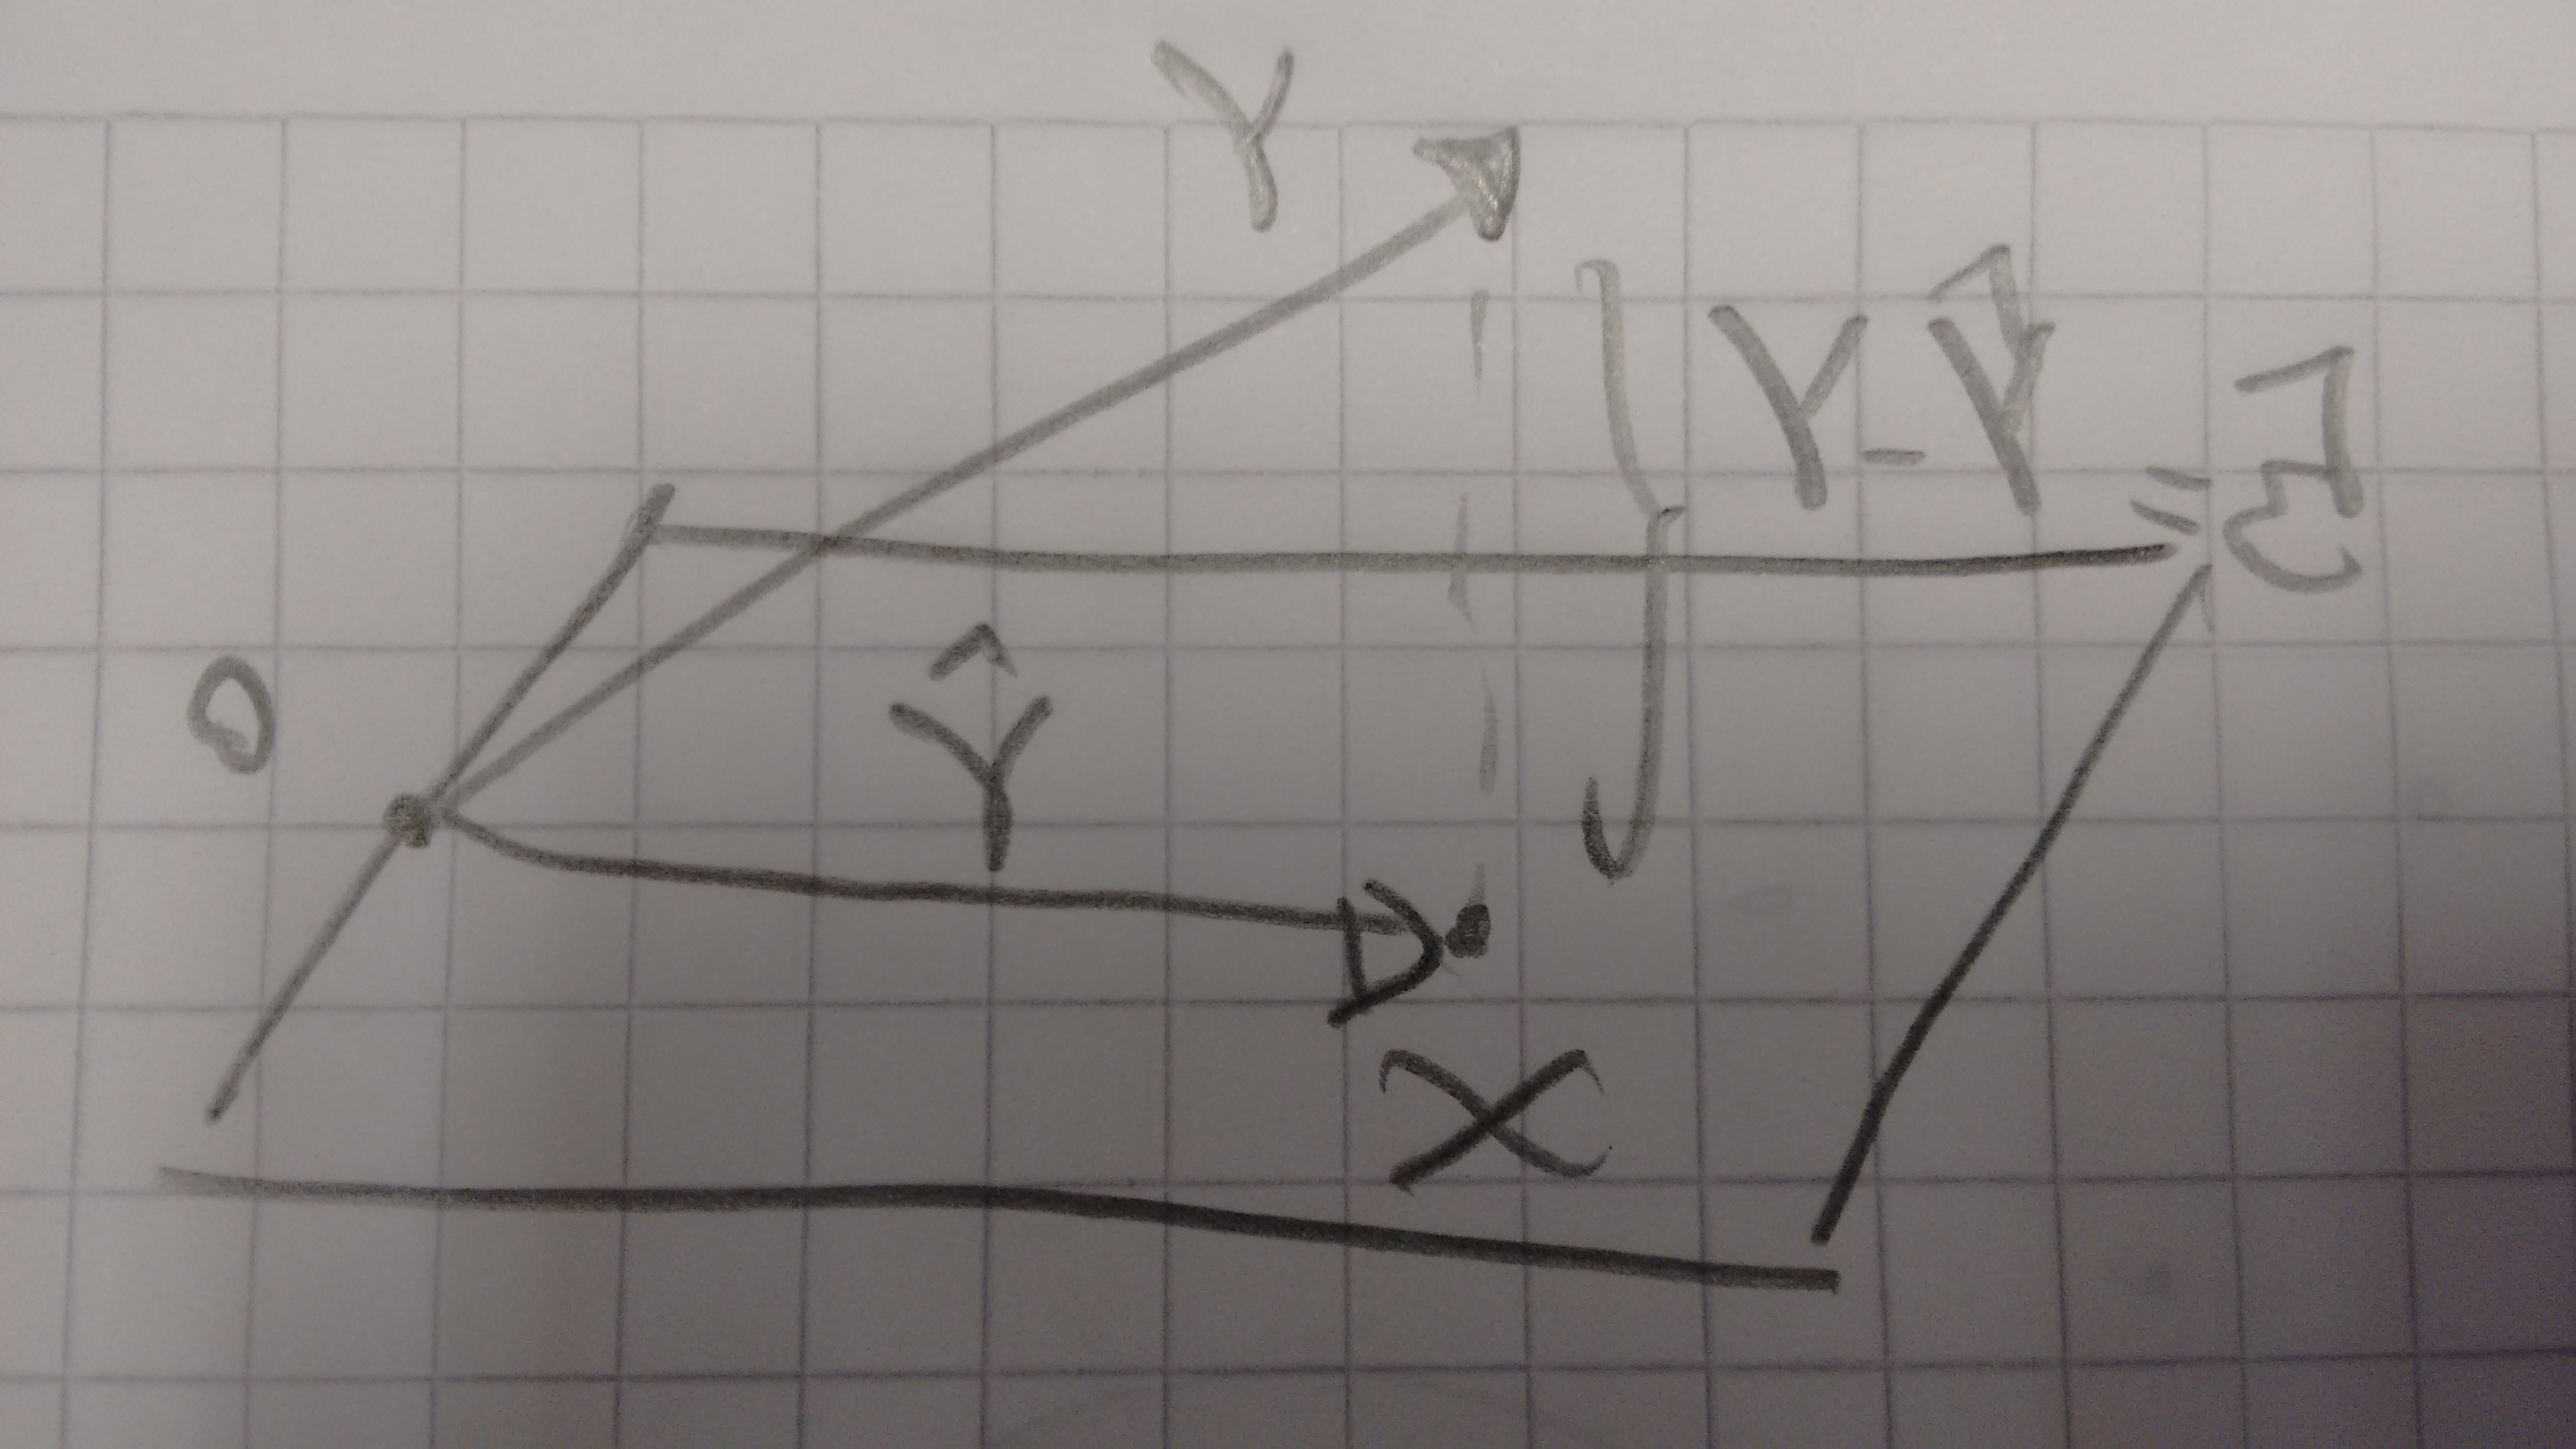
\includegraphics[scale=0.1]{imagenes/proyeccion.jpg}
\end{center}

$\hat{\epsilon} = Y - \hat{Y}$, se llama vector de residuos. Es aleatorio y observable teniendo en cuenta que $\epsilon$ no es observable.


\section{Modelo de Rango Completo}
Suponemos ahora que $rg(X) = k$, es decir, las columnas de $X$ son l.i..\\

Consecuencia de lo anterior es que $dim <X> = k$ y que $X'X$ tiene rango $k$, es decir, resulta invertible porque es $k\times k$.\\
Con esto podemos calcular $\hat{\beta}$, que es único gracias a esta hipótesis. Porque siendo $dim <X> = k$, entonces $\exists ! \hat{\beta} \in \mathbb{R}^k$ tal que $\hat{Y} = X\hat{\beta}$\\

Para el cálculo de $\hat{\beta}$ mostramos que
\begin{align*}
& \hat{\epsilon} = Y - \hat{Y} \perp <X>\\
\Leftrightarrow & (X\beta)'(Y-\hat{Y}) = 0, \forall \beta \in \mathbb{R}^k\\
\Leftrightarrow & X'(Y-\hat{Y}) = 0\\
\Leftrightarrow & X'(Y-X\hat{\beta}) = 0\\
\Rightarrow & (X'X)^{-1}X'Y
\end{align*}
Que es un sistema lineal de ecuaciones ``normales'', aquí obviamente se usa la hipótesis de rango completo.\\

¿Qué propiedades tiene $\hat{\beta}$?
\section{Insesgamiento}
\begin{align*}
\mathbb{E}(\hat{\beta}) &= \mathbb{E}((X'X)^{-1}X'Y)\\
&= (X'X)^{-1}X'\mathbb{E}(Y)\\
\end{align*}
Pero 
\begin{align*}
Y = X\beta + \epsilon \Rightarrow \mathbb{E}(X\beta) + \underbrace{\mathbb{E}(\epsilon)}_{0} = X\beta\\
\Rightarrow \mathbb{E}(\hat{\beta}) = (X'X)^{-1}X'X\beta = \beta
\end{align*}
Luego $\hat{\beta}$ es insesgado.\\

¿Qué pasa con la varianza de $\hat{\beta}$?\\

Debemos definir la varianza de un vector aleatorio.\\

Sea $Z \in \mathbb{R}^n$ un vector aleatorio con componentes $Z_{1}\ldots Z_{n}$ tal que $\mathbb{V}(Z_{i}) < \infty$. O de manera equivalente $\mathbb{E}(Z_{i}^2) < \infty$.\\

Se define la matriz de varianzas-covarianzas de $Z$ como:
\begin{align*}
\mathbb{V}(Z) = (Cov(Z_{i},Z_{j}))_{i,j = 1\ldots n}
\end{align*}
Entonces $\mathbb{V}$ es una matriz simétrica de $n\times n $ (con elementos finitos, por la finitud de segundos momentos).\\
En la diagonal se encuentran las varianzas $\mathbb{V}(Z_{1}), \ldots \mathbb{V}(Z_{n})$.\\

Recordemos que 
\begin{align*}
Cov(Z_{i}, Z_{j}) &= \mathbb{E}(Z_{i}-\mathbb{E} (Z_{i})) (Z_{j}-\mathbb{E} (Z_{j})) \\
&= \mathbb{E}(Z_{i}Z_{j})- \mathbb{E}(Z_{i})\mathbb{E}(Z_{j})
\end{align*}

Con lo anterior podemos escribir
\begin{align*}
\mathbb{V} &= \mathbb{E}((Z-\mathbb{E}(Z))(Z-\mathbb{E}(Z))')
\end{align*}
Por otra parte, si multiplicamos $Z$ por una matriz, digamos $AZ$, entonces
\begin{align*}
\mathbb{V}(AZ) &= \mathbb{E}((Z-\mathbb{E}(Z))(Z-\mathbb{E}(Z))'A')\\
&= A \mathbb{V}(Z)A'
\end{align*}

Es fácil ver que $\mathbb{V}(Z)$ es semidefinida positiva. En efecto:
\begin{align*}
\alpha'\mathbb{V}\alpha = \mathbb{V}(\alpha'Z\alpha) \ge 0
\end{align*}

Volvamos a $\hat{\beta}$. Supongamos ahora que $\epsilon$ tiene segundos momentos finitos, i.e., $\mathbb{E}(\epsilon_{i}^2) < \infty, \forall i = 1\ldots n$. Con esto, sabemos que $\mathbb{\epsilon}$ está definida.\\
Notamos que $\mathbb{V}(\epsilon) = \mathbb{V}(\epsilon\epsilon')$, porque $\mathbb{E}(\epsilon) = 0$.\\
Digamos que $\Sigma = \mathbb{E}(\epsilon\epsilon')$.\\
Recordemos que $\hat{\beta} = (X'X)^{-1}X'Y$.\\
\begin{align*}
\Rightarrow \mathbb{V}(\hat{\beta}) &= \mathbb{V}((X'X)^{-1}X'Y)\\
&= (X'X)^{-1}X' \underbrace{\mathbb{V}(Y)}_{\mathbb{V}(\epsilon)}X(X'X)^{-1}\\
\mathbb{V}(\hat{\beta}) = (X'X)^{-1}X' \Sigma X(X'X)^{-1}
\end{align*}
Agreguemos la hipótesis de errores no correlacionados con igual varianza. Es decir, $\Sigma = \sigma^2 I$ (ojo que esto no significa que los $\epsilon_{i}$ son independientes.\\

En tal caso:
\begin{align*}
\mathbb{V}(\hat{\beta}) &= \sigma^2(X'X)^{-1}\\
\mathbb{V}(\hat{\beta}_{i}) &= \sigma^2 diag(X'X)^{-1}
\end{align*}

Podemos aprovechar que el modelo es de rango completo para calcular los proyectores $P_{X}$ en $<X>$ y $P_{X^{\perp}}$ en $<X>^{\perp}$ (el ortogonal a $<X>$).
\begin{align*}
P_{X}Y = \hat{Y} = X \hat{\beta} = X(X'X)^{-1}X'Y
\end{align*}
es decir $P_{X}= X(X'X)^{-1}X'$ y $P_{X^{\perp}} = I - X(X'X)^{-1}X'$\\

¿Qué tan bueno es $\hat{\beta}$ comparado con otras alternativas de estimación de $\beta$? (Optimalidad)

\section{Teorema de Gauss-Markov}
Se refiere a la optimalidad de $\hat{\beta}$ en la clase de todos los estimadores lineales en $Y$ e insesgados para $\beta$.\\
$\hat{\beta}$ es un estimador de $\beta$ lineal en $Y$, porque se escribe $\hat{\beta} = BY$ con $B=(X'X)^{-1}X'$ matriz.\\
Si consideramos ahora $\tilde{\beta}$ de la forma $\tilde{\beta} = \tilde{B}Y$, insesgado para $\beta$. Será mejor que $\hat{\beta}$? ($\mathbb{V}(\tilde{\beta}) \le \mathbb{V}(\hat{\beta})$ (diferencia definida negativa))\\

Notar que
\begin{align*}
\mathbb{E}(\tilde{\beta})&= \tilde{B}\mathbb{E}(Y)\\
&= \tilde{B}XB = \beta, \forall \beta
\end{align*}

\subsection{Teorema}
Sea $Y=X\beta + \epsilon$, el modelo lineal de rango completo con $\mathbb{E}(\epsilon\epsilon')) = \sigma^2 I$.\\
Entonces $\hat{\beta} = (X'X)^{-1}X'Y$ es el mejor estimador lineal insesgado de $\beta$.\\
En la demostración veremos que se entiende por ``el mejor''.
\subsubsection{Demostración}
Consideremos una combinación lineal de los $\beta_{i}$, digamos $\phi = \sum_{j=1}^{k}a_{j}\beta_{j} = a'\beta, a =\begin{bmatrix}
           a_{1} \\
           a_{2} \\
           \vdots \\
           a_{n}
         \end{bmatrix}$, que nos interesa estimar insesgadamente, mediante la combinación lineal de los $Y_{i}$.\\
         
El estimador de mínimos cuadrados de $\phi$ se define como
\begin{align*}
\hat{\phi} = a'\hat{\beta} = a'(X'X)^{-1}X'Y
\end{align*}
$\hat{\phi}$ es evidentemente lineal en $Y$. Además,
\begin{align*}
\mathbb{E}(\hat{\phi}) = a' \mathbb{E} (\hat{\beta}) = a' \beta = \phi
\end{align*}
Veamosue $\hat{\phi}$ es lineal en $Y$ e insesgado para $\phi$.\\

Sea $\tilde{\phi}$ otro estimador lineal en $Y$, insesgado para $\phi$.\\
Existe entonces $b\in\mathbb{R}^n$ tal que $\tilde{\phi} = b'Y$. Por la condición de insesgamiento
\begin{align*}
& \mathbb{E}(\tilde{\phi}) = b'\mathbb{E}(Y) = b'X\beta = \phi = a'\beta, \forall \beta \in \mathbb{R}^{k}\\
\Leftrightarrow & b'X = a'\\
\Leftrightarrow & a = X'b
\end{align*}
Veamos que lo anterior significa que $a$ es combinación lineal de filas de $X$.\\

Debido a que $rg(X) = k$ (suponiendo $n>k$) entonces $\exists b$ tq $a=X'b$.\\

Pero si $rg(X) < k$, entonces no hay garantía.\\

Calculemos $\mathbb{V}(\hat{\phi})$ y $\mathbb{V}(\tilde{\phi})$ y comparemos.
\begin{align*}
\mathbb{V}(\hat{\phi}) &= \mathbb{V}(a'\hat{\beta})\\
&= a'\mathbb{V}(\hat{\beta})a\\
&= \sigma^2 a'(X'X)^{-1} a\\
\mathbb{V}(\tilde{\phi}) &= \mathbb{V}(b'Y)\\
&= b' \mathbb{V}(Y)b\\
&= \sigma^2 b'b
\end{align*}

Debido a que $a = X'b$ tenemos que 
\begin{align*}
\mathbb{V}(\hat{\phi}) &= \sigma^2 b'\underbrace{X(X'X)^{-1}Z'}_{P_{X}}b'\\
&= \sigma^2 (b'b - b'P_{X})b)\\
&= \sigma^2b'(I-P_{X})b\\
&= \sigma^2 b'P_{X^{\perp}}b \ge 0
\end{align*}
Hemos probado que $\forall a \in \mathbb{R}^{k}$, $\hat{\phi}= a' \hat{\beta}$ es mejor que $\tilde{\phi}= b'Y$ con $a=X'b$.\\

Notar que los $\epsilon$ pueden ser dependientes y tener $\forall$ distribución, a condición de tener $\mathbb{E}(\epsilon)= 0$ y $\mathbb{E}(\epsilon\epsilon') = \sigma^2I$.
\end{document}
